\documentclass{beamer}
\usetheme{Boadilla}
\usepackage{tikz,xcolor,caption,mathabx}
\usetikzlibrary{graphs,graphs.standard}
\captionsetup[figure]{labelformat=empty}

\def\Circlearrowleft{\ensuremath{%
  \rotatebox[origin=c]{180}{$\circlearrowleft$}}}
\def\Circlearrowright{\ensuremath{%
  \rotatebox[origin=c]{180}{$\circlearrowright$}}}
\def\CircleArrowleft{\ensuremath{%
  \reflectbox{\rotatebox[origin=c]{180}{$\circlearrowleft$}}}}
\def\CircleArrowright{\ensuremath{%
  \reflectbox{\rotatebox[origin=c]{180}{$\circlearrowright$}}}}

\usepackage[T1]{fontenc}
\usepackage{concrete}
\usepackage{amsmath,amsthm,amssymb}
\usepackage{multicol}
\usepackage{caption}
\usepackage{subcaption}
%\usepackage{enumitem}
\usepackage{standalone}
\usepackage{tkz-graph}
\usepackage{tikz}

\usetikzlibrary{shapes}
\usepackage{amsfonts}
\usepackage{mathtools}
\usepackage[normalem]{ulem}
\usepackage{adjustbox, centernot}
\usepackage{wrapfig,graphicx}
\theoremstyle{plain}
  \newtheorem{conjecture}{Conjecture}
  \newtheorem{observation}{Observation}
\renewcommand{\rmdefault}{pplx}
\setbeamertemplate{navigation symbols}{}

\newcommand{\GG}{\ensuremath{\mathcal{G}}}
\newcommand{\ZZ}{\ensuremath{\mathbb{Z}}}
\DeclarePairedDelimiter\ceil{\lceil}{\rceil} % Command for ceiling function : \ceil{x}
\DeclarePairedDelimiter\floor{\lfloor}{\rfloor} % Command for floor function: \floor{x}
\newcommand{\Mod}[1]{\ (\mathrm{mod}\ #1)}
\title{Designs for Forests with Seven Edges}
\author{Danny Banegas}
\institute{University of Minnesota: Duluth}
\date{\today}

\begin{document}

\frame{\titlepage}

% Section: Basic Graph Notation
\section{Basic Graph Notation}
\begin{frame}{Graph Fundamentals}
    \begin{itemize}
        \pause
        \item A \textbf{graph} $G = (V, E)$ consists of a set of vertices $V$ and a set of edges $E$.
        \pause
        \item An edge $e \in E$ is a pair of vertices $e = \{u, v\}$ where $u, v \in V$.
        \pause
        \item A \textbf{subgraph} $H$ of $G$ is a graph whose vertices and edges are subsets of $V$ and $E$, respectively.
        \pause
        \item A \textbf{simple graph} is one where two vertices may only share one edge and where no vertex shares an edge with itself.
        
    \end{itemize}
\end{frame}

\begin{frame}{Graph Fundamentals}
    Here is an example of a disconnected simple graph. $G = (V, E)$ where:
    \pause
    \begin{itemize}
        \item $V = \{a, b, c, d, e, f, g, h, i\}$
        \pause
        \item $E = \{\{a, b\}, \{a, c\}, \{a, d\}, \{a, e\}, \{a, f\}, \{a, g\},\{h,i\}\}$
    \end{itemize}
    \pause
    \begin{center}
        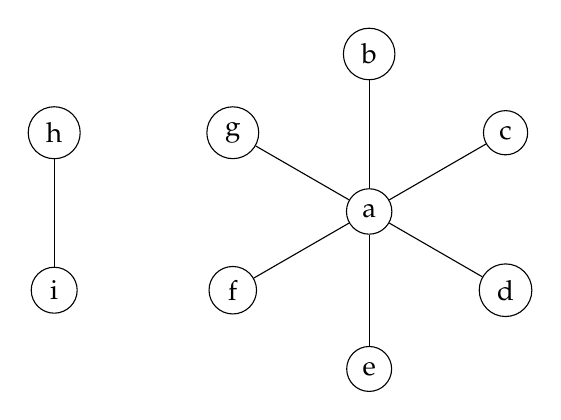
\begin{tikzpicture}[scale=2]
            % Define the vertices in a cycle
            \node (b) at (90:1) [circle, draw] {b};
            \node (c) at (30:1) [circle, draw] {c};
            \node (d) at (330:1) [circle, draw] {d};
            \node (e) at (270:1) [circle, draw] {e};
            \node (f) at (210:1) [circle, draw] {f};
            \node (g) at (150:1) [circle, draw] {g};
            
            % Define the center vertex
            \node (a) at (0,0) [circle, draw] {a};
            
            % Define the lone 2-path
            \node (h) at (-2, 0.5) [circle, draw] {h};
            \node (i) at (-2, -0.5) [circle, draw] {i};
            
            % Draw the edges in a star
            \draw (a) -- (b);
            \draw (a) -- (c);
            \draw (a) -- (d);
            \draw (a) -- (e);
            \draw (a) -- (f);
            \draw (a) -- (g);
            
            % Draw the lone 2-path
            \draw (h) -- (i);
        \end{tikzpicture}
    \end{center}
\end{frame}

% Section: Families of Graphs
\section{Families of Graphs}

% Frame: Cycle Graphs
\begin{frame}{Cycle Graphs}
\pause
    \begin{itemize}
        \item A \textbf{cycle graph} $C_n$ is a graph that consists of a single \textbf{cycle}. A cycle is an internally non-repeating sequence of vertices which starts and ends at the same vertex.
        \pause
        \item It has $n$ vertices and $n$ edges.
        pause
        \item We denote can these cycles using cycle notation like in a symmetric group, $(012345)=(501234)=(450123)=\cdots=(123450)$. The previous cycle is the only one in $C_{6}$ which is shown below.
    \end{itemize}
    \pause
    \begin{figure}
        \centering
        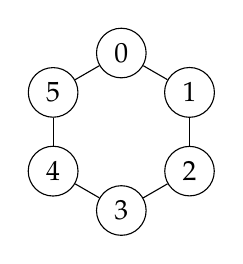
\begin{tikzpicture}
            % Define the vertices
            \node (v1) at (90:1) [circle, draw] {0};
            \node (v2) at (30:1) [circle, draw] {1};
            \node (v3) at (-30:1) [circle, draw] {2};
            \node (v4) at (-90:1) [circle, draw] {3};
            \node (v5) at (-150:1) [circle, draw] {4};
            \node (v6) at (150:1) [circle, draw] {5};
            
            % Draw the edges
            \draw (v1) -- (v2);
            \draw (v2) -- (v3);
            \draw (v3) -- (v4);
            \draw (v4) -- (v5);
            \draw (v5) -- (v6);
            \draw (v6) -- (v1);
        \end{tikzpicture}
        \caption{The Cycle graph $C_6$}
    \end{figure}
\end{frame}

% Frame: Tree Graphs
\begin{frame}{Tree Graphs}
    \pause
    \begin{itemize}
        \item A \textbf{tree graph} is an \textbf{acyclic} connected graph. An acyclic graph is one which contains no cycles.
        \pause
        \item It has $n$ vertices and $n-1$ edges.
    \end{itemize}
    \pause
    \begin{figure}
        \centering
        \begin{tikzpicture}[scale=1.5]
            \node[circle, draw] (a) at (0,0) {};
            \node[circle, draw] (b) at (-1,-1) {};
            \node[circle, draw] (c) at (1,-1) {};
            \node[circle, draw] (d) at (-1.5,-2) {};
            \node[circle, draw] (e) at (-0.5,-2) {};
            \node[circle, draw] (f) at (1.5,-2) {};
            
            \draw (a) -- (b);
            \draw (a) -- (c);
            \draw (b) -- (d);
            \draw (b) -- (e);
            \draw (c) -- (f);
        \end{tikzpicture}
        \caption{A tree graph on $6$ edges}
    \end{figure}
\end{frame}
% Path graphs
\begin{frame}{Path Graphs}
    \pause
    \begin{itemize}
        \item A \textbf{path graph} is a special type of tree graph. It is simply a graph that can be described completely by a sequence of vertices.
        \pause
        \item It has $n$ vertices and $n-1$ edges.
    \end{itemize}

    \begin{figure}
        \centering
        \begin{tikzpicture}[scale=1.5]
            \node[circle, draw] (a) at (0,0) {};
            \node[circle, draw] (b) at (-1,-1) {};
            \node[circle, draw] (c) at (1,-1) {};
            \node[circle, draw] (d) at (-1.5,-2) {};
            \node[circle, draw] (f) at (1.5,-2) {};
            
            \draw (a) -- (b);
            \draw (a) -- (c);
            \draw (b) -- (d);
            \draw (c) -- (f);
        \end{tikzpicture}
        \caption{A path graph on $6$ edges}
    \end{figure}
\end{frame}

% Frame: Forest Graphs
\begin{frame}{Forest Graphs}
    \begin{itemize}
    \pause
        \item A \textbf{forest} is a disjoint union of trees.
        \pause
        \item It consists of multiple components, each being a tree.
    \end{itemize}
    \pause
    \begin{figure}
        \centering
        \begin{tikzpicture}[scale=1.5]
            % Tree 1
            \node[circle, draw] (a1) at (0,0) {};
            \node[circle, draw] (b1) at (-0.5,-1) {};
            \node[circle, draw] (c1) at (0.5,-1) {};
            \draw (a1) -- (b1);
            \draw (a1) -- (c1);
            
            % Tree 2
            \node[circle, draw] (a2) at (2,0) {};
            \node[circle, draw] (b2) at (1.5,-1) {};
            \node[circle, draw] (c2) at (2.5,-1) {};
            \node[circle, draw] (d2) at (2,-2) {};
            \draw (a2) -- (b2);
            \draw (a2) -- (c2);
            \draw (c2) -- (d2);
        \end{tikzpicture}
        \caption{A Forest graph composed of trees with $3$ and $4$ vertices, respectively }
    \end{figure}
\end{frame}

% Frame 1: Complete Graphs
\begin{frame}{Complete Graphs}
\pause
    \begin{itemize}
        \item The \textbf{complete graph} $K_n$ is one where every pair of distinct vertices is connected by a unique edge.
        \pause
        \item It has $n$ vertices and \textcolor{red}{how many edges?}
    \end{itemize}
    \pause
    \begin{figure}
    \begin{center}
        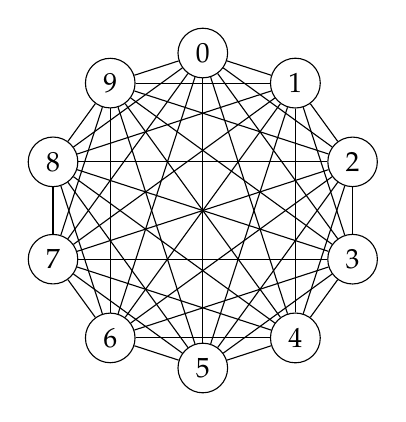
\begin{tikzpicture}[scale = 3]
            \graph[nodes={draw, circle}, n=10, clockwise, radius=2cm]
            { subgraph K_n [V={0,1,2,3,4,5,6,7,8,9}];};
        \end{tikzpicture}
    \end{center}
    \caption{The Complete graph $K_{10}$}
    \end{figure}
\end{frame}
%frame 2
\begin{frame}{Complete Graphs}
    \begin{itemize}
        \item The \textbf{complete graph} $K_n$ is one where every pair of distinct vertices is connected by a unique edge.
        \item It has $n$ vertices and \textcolor{blue}{$\binom{n}{2}$} edges.
    \end{itemize}

    \begin{figure}
    \begin{center}
        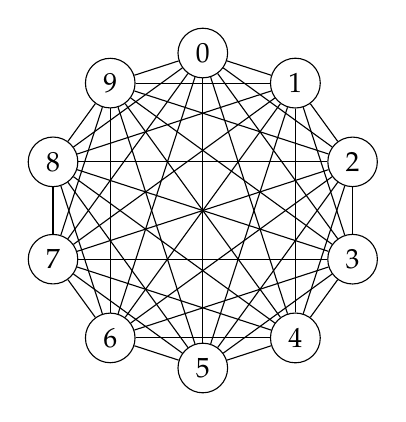
\begin{tikzpicture}[scale = 3]
            \graph[nodes={draw, circle}, n=10, clockwise, radius=2cm]
            { subgraph K_n [V={0,1,2,3,4,5,6,7,8,9}];};
        \end{tikzpicture}
    \end{center}
    \caption{The Complete graph $K_{10}$}
    \end{figure}
\end{frame}

% Section: Graph Decomposition
\section{Graph Decomposition}
%Frame 1
\begin{frame}{Graph Decompositions}
\pause
    \begin{itemize}
        \item Let $K$ be a simple graph. A \textbf{decomposition} of $K$ is a collection of pairwise edge disjoint subgraphs $\GG = \{G_{0}, G_{1}, \hdots, G_{m}\}$ such that every edge of $K$ belongs to exactly one member of $\GG$.
        \pause
        \item We call such a collection of subgraphs a decomposition because their union is the entire graph.
    \end{itemize}
        \pause
    \begin{figure}
        \begin{center}
            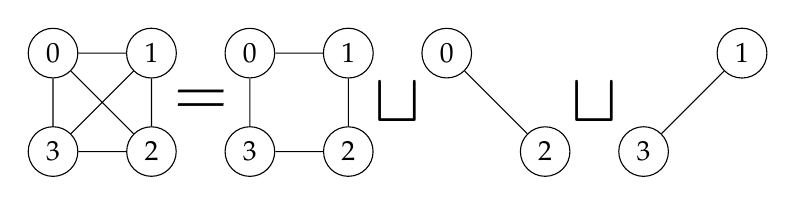
\begin{tikzpicture}[scale=1.25]
                % First graph
                \node (0) at (0, 0) [circle, draw] {0};
                \node (1) at (1, 0) [circle, draw] {1};
                \node (2) at (1, -1) [circle, draw] {2};
                \node (3) at (0, -1) [circle, draw] {3};
    
                \draw (2) -- (3) -- (0) -- (1);
                \draw (0) -- (2) -- (1) -- (3);
                \pause
                % "=" symbol
                \node at (1.5, -0.5) {\Huge $=$};
                % Second graph
                \pause
                \begin{scope}[xshift=2cm]
                    \node (0) at (0, 0) [circle, draw] {0};
                    \node (1) at (1, 0) [circle, draw] {1};
                    \node (2) at (1, -1) [circle, draw] {2};
                    \node (3) at (0, -1) [circle, draw] {3};
    
                    \draw (0) -- (1) -- (2) -- (3) -- (0);
                \end{scope}
                \pause
                % "\cup" symbol
                \node at (3.5, -0.5) {\Huge $\sqcup$};
                
                % Third graph
                \begin{scope}[xshift=4cm]
                    \node (0) at (0, 0) [circle, draw] {0};
                    
                    \node (2) at (1, -1) [circle, draw] {2};
                    
    
                    \draw (0) -- (2);
                    
                \end{scope}
                \pause
                \node at (5.5, -0.5) {\Huge $\sqcup$};
                %Fourth graph
                \begin{scope}[xshift=6cm]
                    
                    \node (1) at (1, 0) [circle, draw] {1};
                    
                    \node (3) at (0, -1) [circle, draw] {3};
    
                    
                    \draw (1) -- (3);
                \end{scope}
            \end{tikzpicture}
        \end{center}
        \caption{Decomposition of $K_4$ into a $C_4$ and two $P_2$'s}
    \end{figure}
\end{frame}

% Section: G-Decomposition
\section{G-Decompositions}
%frame 1
\begin{frame}{Designs}
    \pause
    \begin{itemize}
        \item Let $\GG = \{G_{0}, G_{1}, \hdots, G_{m}\}$ be a decomposition of some graph $K$.
        \pause
        \item If every subgraph in $\GG$ is isomorphic to some graph $G$, then we call $\GG$ a $G-$decomposition of $K$ and say that $K$ allows a $G-$decomposition or \textbf{$(K,G)-$design}.
        \pause
        \item If $K\cong K_{n}$ then we call $\GG$ a \textbf{$G-$design} of order $n$.
        \pause
    \end{itemize}
    \begin{figure}
        \begin{center}
            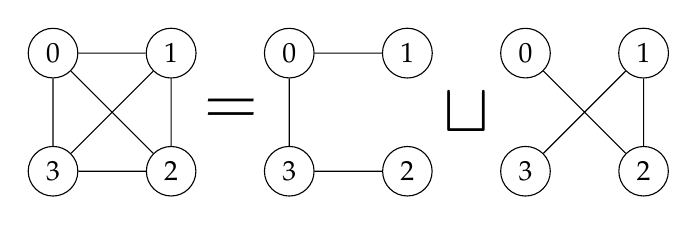
\begin{tikzpicture}[scale=1.5]
                % First graph
                \node (0) at (0, 0) [circle, draw] {0};
                \node (1) at (1, 0) [circle, draw] {1};
                \node (2) at (1, -1) [circle, draw] {2};
                \node (3) at (0, -1) [circle, draw] {3};
    
                \draw (2) -- (3) -- (0) -- (1);
                \draw (0) -- (2) -- (1) -- (3);
                \pause
                % "=" symbol
                \node at (1.5, -0.5) {\Huge $=$};
    
                % Second graph
                \begin{scope}[xshift=2cm]
                    \node (0) at (0, 0) [circle, draw] {0};
                    \node (1) at (1, 0) [circle, draw] {1};
                    \node (2) at (1, -1) [circle, draw] {2};
                    \node (3) at (0, -1) [circle, draw] {3};
    
                    \draw (1) -- (0) -- (3) -- (2);
                \end{scope}
                \pause
                % "\cup" symbol
                \node at (3.5, -0.5) {\Huge $\sqcup$};
                
                \begin{scope}[xshift=4cm]
                    \node (0) at (0, 0) [circle, draw] {0};
                    \node (1) at (1, 0) [circle, draw] {1};
                    \node (2) at (1, -1) [circle, draw] {2};
                    \node (3) at (0, -1) [circle, draw] {3};
                    
                    \draw (0) -- (2) -- (1) -- (3);
                \end{scope}
            \end{tikzpicture}
        \end{center}
        \caption{A $P_{3}-$Design of order $4$}
    \end{figure}
\end{frame}

%necessary conditions
\begin{frame}{Necessary condition}
\begin{itemize}
\item Let $G$ be a graph on $m$ edges. Then there exists a $(K,G)-$design only if $m$ divides $|E(G)|$.
\pause
\item If $K\cong K_{n}$, then there exists a $(K,G)-$design only if $m$ divides $\binom{n}{2}=\frac{n(n-1)}{2}$.
\pause
\item Equivalently, there exists a $G-$design of order $n$ only if $n$ is idempotent modulo $2m$.  This is easy to show.
\pause
\end{itemize}

\begin{block}{Proof}
    Let $m,n\in \mathbb{N}$. Suppose $m \mid \binom{n}{2}$. Then $\frac{n(n-1)}{2} = mq$ for some $q \in \mathbb{N}$. So then $\frac{n(n-1)}{2m} = q$, and thus $n(n-1) \equiv 0 \pmod{2m}$. Therefore $n \equiv n^2 \pmod{2m}$, and so $n$ is idempotent modulo $2m$. Suppose $n$ is idempotent modulo $2m$, then $n^{2}>n$ and therefore $n^{2}-n=n(n-1)=2mp$ for some $p\in \mathbb{N}$. So then $\frac{n(n-1)}{2}=\binom{n}{2}=mp$ and $m$ divides $\binom{n}{2}._{\;\;\qedsymbol}$ 
    \end{block}
\end{frame}
% cyclic designs
\section{cyclic designs}
\begin{frame}{Cyclic designs}
    \pause
    \begin{itemize}
    \item Let $V(K_n)=\mathbb{Z}_n$
    \pause
    \item A $G$-design is \emph{cyclic} if the permutation $v\mapsto v+1$ on $V(K_n)$ is an automorphism of the design.
    \pause
    \item We call this act of applying permutations to a labeling \emph{clicking}.
    \end{itemize}
    \end{frame}

%nodes placed---------------------------------------------------------------------
\begin{frame}{An example of a cyclic design}
    \textbf{Cyclic $P_3$-design of order 5}\\

    \begin{figure}
        \centering
        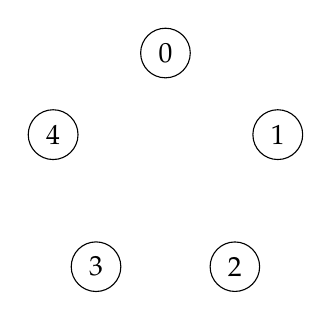
\begin{tikzpicture}[scale=1.5]
            % Define the vertices
            \node[circle, draw=black, fill=white, text=black] (0) at (90:1) {0};
            \node[circle, draw=black, fill=white, text=black] (1) at (18:1) {1};
            \node[circle, draw=black, fill=white, text=black] (2) at (306:1) {2};
            \node[circle, draw=black, fill=white, text=black] (3) at (234:1) {3};
            \node[circle, draw=black, fill=white, text=black] (4) at (162:1) {4};
            
        \end{tikzpicture}
    \end{figure}
\end{frame}
%click black----------------------------------------------------------------------
\begin{frame}{An example of a cyclic design}
    \textbf{Cyclic $P_3$-design of order 5}\\
    \color{black} $\{1,0,3\}$ \newline
    
    \begin{figure}
        \centering
        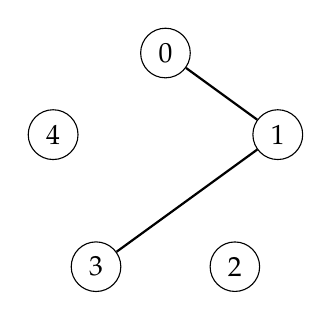
\begin{tikzpicture}[scale=1.5]
            % Define the vertices
            \node[circle, draw=black, fill=white, text=black] (0) at (90:1) {0};
            \node[circle, draw=black, fill=white, text=black] (1) at (18:1) {1};
            \node[circle, draw=black, fill=white, text=black] (2) at (306:1) {2};
            \node[circle, draw=black, fill=white, text=black] (3) at (234:1) {3};
            \node[circle, draw=black, fill=white, text=black] (4) at (162:1) {4};
            
            % Draw the edges of the P_3 subgraphs
            \draw[black, thick] (0) -- (1) -- (3);
        \end{tikzpicture}
    \end{figure}
\end{frame}
%click red------------------------------------------------------------------------
\begin{frame}{An example of a cyclic design}
    \textbf{Cyclic $P_3$-design of order 5}\\
    \color{black} $\{1,0,3\}$ \newline
    \color{red} $\{2,1,4\}$ \newline

    \begin{figure}
        \centering
        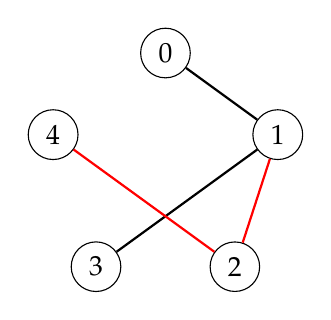
\begin{tikzpicture}[scale=1.5]
            % Define the vertices
            \node[circle, draw=black, fill=white, text=black] (0) at (90:1) {0};
            \node[circle, draw=black, fill=white, text=black] (1) at (18:1) {1};
            \node[circle, draw=black, fill=white, text=black] (2) at (306:1) {2};
            \node[circle, draw=black, fill=white, text=black] (3) at (234:1) {3};
            \node[circle, draw=black, fill=white, text=black] (4) at (162:1) {4};
            
            % Draw the edges of the P_3 subgraphs
            \draw[black, thick] (0) -- (1) -- (3);
            \draw[red, thick] (1) -- (2) -- (4);
        \end{tikzpicture}
    \end{figure}
\end{frame}
%click blue-----------------------------------------------------------------------
\begin{frame}{An example of a cyclic design}
    \textbf{Cyclic $P_3$-design of order 5}\\
    \color{black} $\{1,0,3\}$ \newline
    \color{red} $\{2,1,4\}$ \newline
    \color{blue} $\{3,2,0\}$ \newline

    \begin{figure}
        \centering
        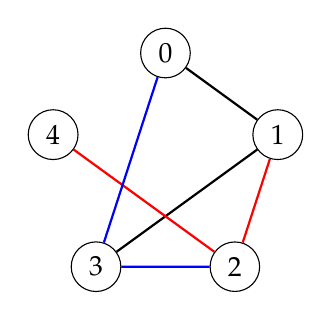
\begin{tikzpicture}[scale=1.5]
            % Define the vertices
            \node[circle, draw=black, fill=white, text=black] (0) at (90:1) {0};
            \node[circle, draw=black, fill=white, text=black] (1) at (18:1) {1};
            \node[circle, draw=black, fill=white, text=black] (2) at (306:1) {2};
            \node[circle, draw=black, fill=white, text=black] (3) at (234:1) {3};
            \node[circle, draw=black, fill=white, text=black] (4) at (162:1) {4};
            
            % Draw the edges of the P_3 subgraphs
            \draw[black, thick] (0) -- (1) -- (3);
            \draw[red, thick] (1) -- (2) -- (4);
            \draw[blue, thick] (2) -- (3) -- (0);
        \end{tikzpicture}
    \end{figure}
\end{frame}
%click green--------------------------------------------------------------------
\begin{frame}{An example of a cyclic design}
    \textbf{Cyclic $P_3$-design of order 5}\\
    \color{black} $\{1,0,3\}$ \newline
    \color{red} $\{2,1,4\}$ \newline
    \color{blue} $\{3,2,0\}$ \newline
    \color{green} $\{4,3,1\}$ \newline

    \begin{figure}
        \centering
        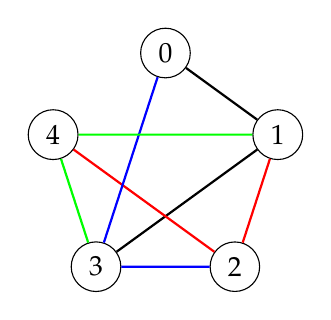
\begin{tikzpicture}[scale=1.5]
            % Define the vertices
            \node[circle, draw=black, fill=white, text=black] (0) at (90:1) {0};
            \node[circle, draw=black, fill=white, text=black] (1) at (18:1) {1};
            \node[circle, draw=black, fill=white, text=black] (2) at (306:1) {2};
            \node[circle, draw=black, fill=white, text=black] (3) at (234:1) {3};
            \node[circle, draw=black, fill=white, text=black] (4) at (162:1) {4};
            
            % Draw the edges of the P_3 subgraphs
            \draw[black, thick] (0) -- (1) -- (3);
            \draw[red, thick] (1) -- (2) -- (4);
            \draw[blue, thick] (2) -- (3) -- (0);
            \draw[green, thick] (3) -- (4) -- (1);
        \end{tikzpicture}
    \end{figure}
\end{frame}
%click magenta--------------------------------------------------------------------
\begin{frame}{An example of a cyclic design}
    \textbf{Cyclic $P_3$-design of order 5}\\
    \color{black} $\{1,0,3\}$ \newline
    \color{red} $\{2,1,4\}$ \newline
    \color{blue} $\{3,2,0\}$ \newline
    \color{green} $\{4,3,1\}$ \newline
    \color{magenta} $\{0,4,2\}$

    \begin{figure}
        \centering
        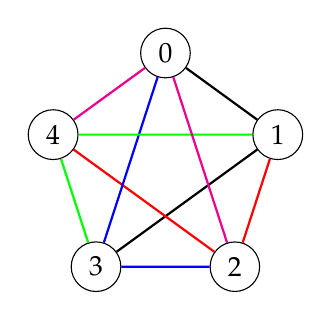
\begin{tikzpicture}[scale=1.5]
            % Define the vertices
            \node[circle, draw=black, fill=white, text=black] (0) at (90:1) {0};
            \node[circle, draw=black, fill=white, text=black] (1) at (18:1) {1};
            \node[circle, draw=black, fill=white, text=black] (2) at (306:1) {2};
            \node[circle, draw=black, fill=white, text=black] (3) at (234:1) {3};
            \node[circle, draw=black, fill=white, text=black] (4) at (162:1) {4};
            
            % Draw the edges of the P_3 subgraphs
            \draw[black, thick] (0) -- (1) -- (3);
            \draw[red, thick] (1) -- (2) -- (4);
            \draw[blue, thick] (2) -- (3) -- (0);
            \draw[green, thick] (3) -- (4) -- (1);
            \draw[magenta, thick] (4) -- (0) -- (2);
        \end{tikzpicture}
        \caption{Cyclic $P_3$-design of order 5}
    \end{figure}
\end{frame}

\section{Edge Length}
\begin{frame}{Edge length}
\begin{itemize}
\item Let $V(K_n)=\{0,1,\hdots,n-1\}$ 
\pause
\item The \emph{length} of edge $xy \in E(K_n)$ is $\min(|x-y|,n-|x-y|)$
\pause
\item If the length of $xy$ is $n-|x-y|\text{ or equivalently, if } |x-y|>\floor{\frac{n}{2}},$ then we call $xy$ a \emph{wrap-around} edge
\end{itemize}
\end{frame}
%frame for example of edge lengths
\begin{frame}{Edge lengths of $K_7$}
\begin{itemize}
\item \color{black} length 1
%\color{blue} length 2 \newline
%\color{red} length 3 \newline
\end{itemize}

\begin{center}
    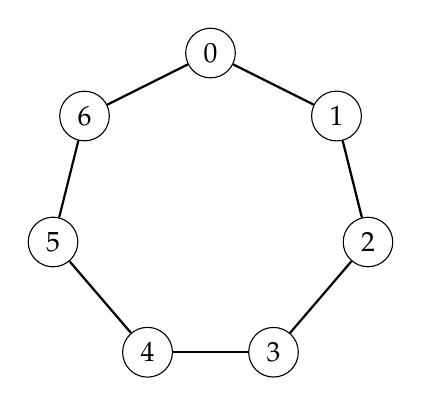
\begin{tikzpicture}[scale=0.2]
   
 \node[circle, draw=black, fill=white, text=black](0) at (0,10) {0};
 \node[circle, draw=black, fill=white, text=black](1) at (8,6) {1};
 \node[circle, draw=black, fill=white, text=black](2) at (10,-2) {2};
 \node[circle, draw=black, fill=white, text=black](3) at (4,-9) {3};
 \node[circle, draw=black, fill=white, text=black](4) at (-4,-9) {4};
 \node[circle, draw=black, fill=white, text=black](5) at (-10,-2) {5};
 \node[circle, draw=black, fill=white, text=black](6) at (-8,6) {6};
 
    %length 1 edges
        \draw[black, thick](0)--(1);
        \draw[black, thick](1)--(2);
        \draw[black, thick](2)--(3);
        \draw[black, thick](3)--(4);
        \draw[black, thick](4)--(5);
        \draw[black, thick](5)--(6);
	  \draw[black, thick](6)--(0);
    \end{tikzpicture}
\end{center}
\end{frame}
%-------------------length 2--------------------------
\begin{frame}{Edge lengths of $K_7$}
\begin{itemize}
\item \color{black} length 1 
\item \color{blue} length 2 
%\color{red} length 3 \newline
\end{itemize}

\begin{center}
    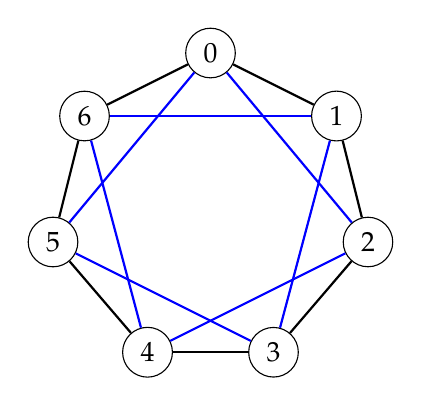
\begin{tikzpicture}[scale=0.2]
   
 \node[circle, draw=black, fill=white, text=black](0) at (0,10) {0};
 \node[circle, draw=black, fill=white, text=black](1) at (8,6) {1};
 \node[circle, draw=black, fill=white, text=black](2) at (10,-2) {2};
 \node[circle, draw=black, fill=white, text=black](3) at (4,-9) {3};
 \node[circle, draw=black, fill=white, text=black](4) at (-4,-9) {4};
 \node[circle, draw=black, fill=white, text=black](5) at (-10,-2) {5};
 \node[circle, draw=black, fill=white, text=black](6) at (-8,6) {6};
 
    %length 1 edges
        \draw[black, thick](0)--(1);
        \draw[black, thick](1)--(2);
        \draw[black, thick](2)--(3);
        \draw[black, thick](3)--(4);
        \draw[black, thick](4)--(5);
        \draw[black, thick](5)--(6);
	  \draw[black, thick](6)--(0); 
%length 2 edges
        \draw[blue, thick](0)--(2);
        \draw[blue, thick](2)--(4);
        \draw[blue, thick](4)--(6);
        \draw[blue, thick](6)--(1);
        \draw[blue, thick](3)--(5);
        \draw[blue, thick](3)--(1);
        \draw[blue, thick](5)--(0);

    \end{tikzpicture}
\end{center}
\end{frame}
%---------------length 3-----------------
\begin{frame}{Edge lengths of $K_{7}$}
\begin{itemize}
\item \color{black} length 1 
\item \color{blue} length 2 
\item \color{red} length 3 
\end{itemize}

\begin{center}
    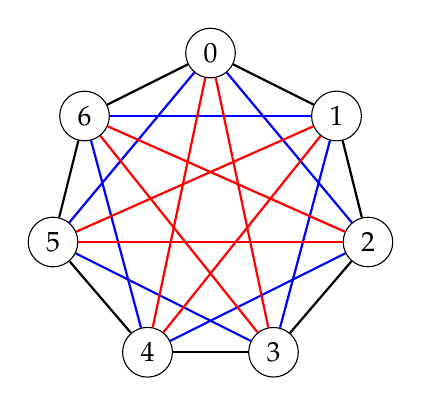
\begin{tikzpicture}[scale=0.2]
   
 \node[circle, draw=black, fill=white, text=black](0) at (0,10) {0};
 \node[circle, draw=black, fill=white, text=black](1) at (8,6) {1};
 \node[circle, draw=black, fill=white, text=black](2) at (10,-2) {2};
 \node[circle, draw=black, fill=white, text=black](3) at (4,-9) {3};
 \node[circle, draw=black, fill=white, text=black](4) at (-4,-9) {4};
 \node[circle, draw=black, fill=white, text=black](5) at (-10,-2) {5};
 \node[circle, draw=black, fill=white, text=black](6) at (-8,6) {6};
 
    %length 1 edges
        \draw[black, thick](0)--(1);
        \draw[black, thick](1)--(2);
        \draw[black, thick](2)--(3);
        \draw[black, thick](3)--(4);
        \draw[black, thick](4)--(5);
        \draw[black, thick](5)--(6);
	    \draw[black, thick](6)--(0); 
%length 2 edges
        \draw[blue, thick](0)--(2);
        \draw[blue, thick](2)--(4);
        \draw[blue, thick](4)--(6);
        \draw[blue, thick](6)--(1);
        \draw[blue, thick](3)--(5);
        \draw[blue, thick](3)--(1);
        \draw[blue, thick](5)--(0);

%length 3 edges
        \draw[red, thick](0)--(3);
        \draw[red, thick](3)--(6);
        \draw[red, thick](6)--(2);
        \draw[red, thick](2)--(5);
        \draw[red, thick](1)--(5);
        \draw[red, thick](1)--(4);
        \draw[red, thick](4)--(0);

    \end{tikzpicture}
\end{center}
\end{frame}
\section{Edge Length and Cyclic Decomposition}
\begin{frame}{Edge Length and Cyclic Decomposition}
    \begin{itemize}
        \item Notice that edge length is preserved by the permutation $v\mapsto v+1$ on $V(K_n)$
        \pause
        \item Also, when $n$ is odd, edge length partitions $E(K_n)$ into $\frac{n-1}{2}$ (the number of lengths) sets of size $n$ (the number of edges of each length) 
        \pause
    \end{itemize}
    \begin{center}
        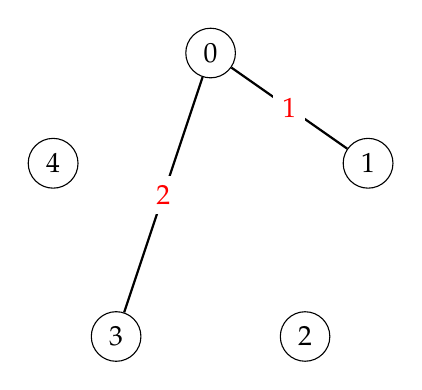
\begin{tikzpicture}[scale=0.2]
       
        
     \node[circle, draw=black, fill=white, text=black](0) at (0,10) {0};
     \node[circle, draw=black, fill=white, text=black](1) at (10,3) {1};
     \node[circle, draw=black, fill=white, text=black](2) at (6,-8) {2};
     \node[circle, draw=black, fill=white, text=black](3) at (-6,-8) {3};
     \node[circle, draw=black, fill=white, text=black](4) at (-10,3) {4};
    \tikzset{EdgeStyle/.style={}} 
        \draw[black, thick] (0) -- (1) node[midway, text=red, fill=white] {1};
        \draw[black, thick] (0) -- (3) node[midway, text=red, fill=white] {2};
        
        \end{tikzpicture}
    \end{center}
        
    \end{frame}
    %-----------click-----
    \begin{frame}
    \frametitle{Edge Length and Cyclic Decomposition}
    \begin{itemize}
        \item Notice that edge length is preserved by the permutation $v\mapsto v+1$ on $V(K_n)$
        \item Also, when $n$ is odd, edge length partitions $E(K_n)$ into $\frac{n-1}{2}$ (the number of lengths) sets of size $n$ (the number of edges of each length) 
    \end{itemize}
    \begin{center}
        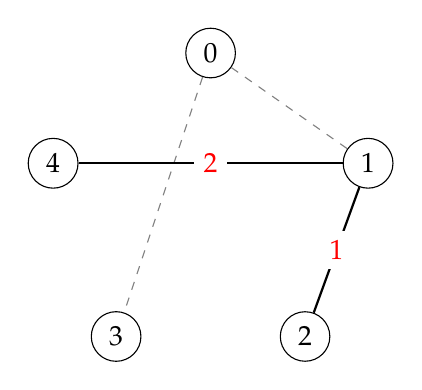
\begin{tikzpicture}[scale=0.2]
       
        
     \node[circle, draw=black, fill=white, text=black](0) at (0,10) {0};
     \node[circle, draw=black, fill=white, text=black](1) at (10,3) {1};
     \node[circle, draw=black, fill=white, text=black](2) at (6,-8) {2};
     \node[circle, draw=black, fill=white, text=black](3) at (-6,-8) {3};
     \node[circle, draw=black, fill=white, text=black](4) at (-10,3) {4};
     
            \draw[gray, dashed](0)--(1);
            \draw[gray, dashed](0)--(3);
            \tikzset{EdgeStyle/.style={}} 
            \draw[black, thick] (4) -- (1) node[midway, text=red, fill=white] {2};
            \draw[black, thick] (1) -- (2) node[midway, text=red, fill=white] {1};
          
        \end{tikzpicture}
    \end{center}
        
    \end{frame}
    %-click---------------
    \begin{frame}
    \frametitle{Edge Length and Cyclic Decomposition}
    \begin{itemize}
        \item Notice that edge length is preserved by the permutation $v\mapsto v+1$ on $V(K_n)$
        \item Also, when $n$ is odd, edge length partitions $E(K_n)$ into $\frac{n-1}{2}$ (the number of lengths) sets of size $n$ (the number of edges of each length) 
    \end{itemize}
    \begin{center}
        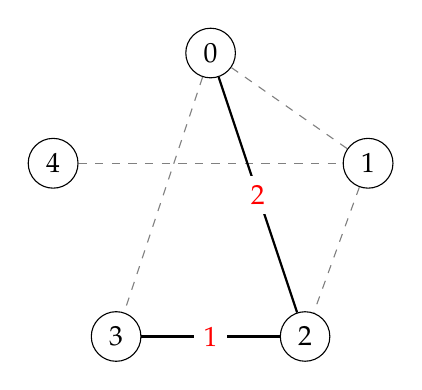
\begin{tikzpicture}[scale=0.2]
       
        
     \node[circle, draw=black, fill=white, text=black](0) at (0,10) {0};
     \node[circle, draw=black, fill=white, text=black](1) at (10,3) {1};
     \node[circle, draw=black, fill=white, text=black](2) at (6,-8) {2};
     \node[circle, draw=black, fill=white, text=black](3) at (-6,-8) {3};
     \node[circle, draw=black, fill=white, text=black](4) at (-10,3) {4};
     
            \draw[gray, dashed](0)--(1);
            \draw[gray, dashed](0)--(3);
     
            \draw[gray, dashed](4)--(1);
            \draw[gray, dashed](1)--(2);
    \tikzset{EdgeStyle/.style={}} 
            \draw[black, thick] (0) -- (2) node[midway, text=red, fill=white] {2};
            \draw[black, thick] (3) -- (2) node[midway, text=red, fill=white] {1};
        \end{tikzpicture}
    \end{center}
        
    \end{frame}
    %---click-----------
    \begin{frame}
    \frametitle{Edge Length and Cyclic Decomposition}
    \begin{itemize}
        \item Notice that edge length is preserved by the permutation $v\mapsto v+1$ on $V(K_n)$
        \item Also, when $n$ is odd, edge length partitions $E(K_n)$ into $\frac{n-1}{2}$ (the number of lengths) sets of size $n$ (the number of edges of each length) 
    \end{itemize}
    \begin{center}
        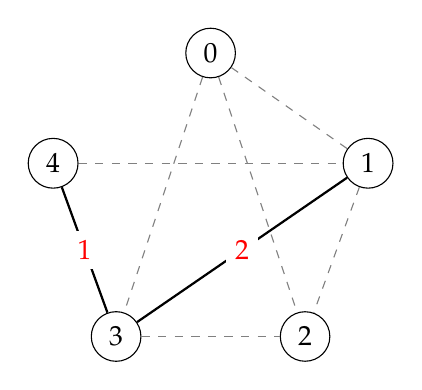
\begin{tikzpicture}[scale=0.2]
       
        
     \node[circle, draw=black, fill=white, text=black](0) at (0,10) {0};
     \node[circle, draw=black, fill=white, text=black](1) at (10,3) {1};
     \node[circle, draw=black, fill=white, text=black](2) at (6,-8) {2};
     \node[circle, draw=black, fill=white, text=black](3) at (-6,-8) {3};
     \node[circle, draw=black, fill=white, text=black](4) at (-10,3) {4};
      
            \draw[gray, dashed](0)--(1);
            \draw[gray, dashed](0)--(3);
             
            \draw[gray, dashed](4)--(1);
            \draw[gray, dashed](1)--(2);
           
            \draw[gray, dashed](0)--(2);
            \draw[gray, dashed](3)--(2);
    \tikzset{EdgeStyle/.style={}}         
        \draw[black, thick] (1) -- (3) node[midway, text=red, fill=white] {2};
        \draw[black, thick] (3) -- (4) node[midway, text=red, fill=white] {1};
          
        \end{tikzpicture}
    \end{center}
        
    \end{frame}
    %----click------
    \begin{frame}
    \frametitle{Edge Length and Cyclic Decomposition}
    \begin{itemize}
        \item Notice that edge length is preserved by the permutation $v\mapsto v+1$ on $V(K_n)$
        \item Also, when $n$ is odd, edge length partitions $E(K_n)$ into $\frac{n-1}{2}$ (the number of lengths) sets of size $n$ (the number of edges of each length) 
    \end{itemize}
    \begin{center}
        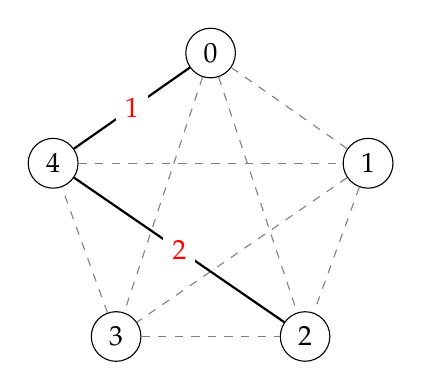
\begin{tikzpicture}[scale=0.2]
       
        
     \node[circle, draw=black, fill=white, text=black](0) at (0,10) {0};
     \node[circle, draw=black, fill=white, text=black](1) at (10,3) {1};
     \node[circle, draw=black, fill=white, text=black](2) at (6,-8) {2};
     \node[circle, draw=black, fill=white, text=black](3) at (-6,-8) {3};
     \node[circle, draw=black, fill=white, text=black](4) at (-10,3) {4};
     
            \draw[gray, dashed](0)--(1);
            \draw[gray, dashed](0)--(3);
     
            \draw[gray, dashed](4)--(1);
            \draw[gray, dashed](1)--(2);
           
            \draw[gray, dashed](0)--(2);
            \draw[gray, dashed](3)--(2);

            \draw[gray, dashed](1)--(3);
            \draw[gray, dashed](3)--(4);

     \tikzset{EdgeStyle/.style={}}    
            \draw[black, thick] (2) -- (4) node[midway, text=red, fill=white] {2};
            \draw[black, thick] (0) -- (4) node[midway, text=red, fill=white] {1};
        \end{tikzpicture}
    \end{center}
        
    \end{frame}
    %----click------
    \begin{frame}{Edge Length and Cyclic Decomposition}
    \begin{itemize}
        \item Notice that edge length is preserved by the permutation $v\mapsto v+1$ on $V(K_n)$
        \item Also, when $n$ is odd, edge length partitions $E(K_n)$ into $\frac{n-1}{2}$ (the number of lengths) sets of size $n$ (the number of edges of each length) 
    \end{itemize}
    \begin{center}
        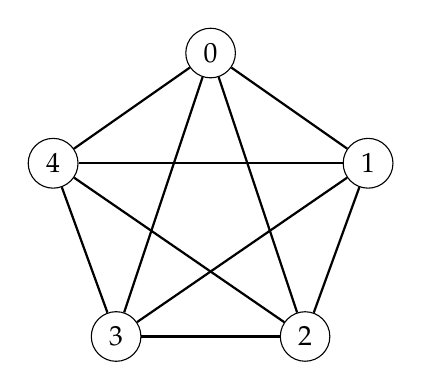
\begin{tikzpicture}[scale=0.2]
    
     \node[circle, draw=black, fill=white, text=black](0) at (0,10) {0};
     \node[circle, draw=black, fill=white, text=black](1) at (10,3) {1};
     \node[circle, draw=black, fill=white, text=black](2) at (6,-8) {2};
     \node[circle, draw=black, fill=white, text=black](3) at (-6,-8) {3};
     \node[circle, draw=black, fill=white, text=black](4) at (-10,3) {4};

            \draw[black, thick](0)--(1);
            \draw[black, thick](0)--(3);

            \draw[black, thick](4)--(1);
            \draw[black, thick](1)--(2);
      
            \draw[black, thick](0)--(2);
            \draw[black, thick](3)--(2);
    
            \draw[black, thick](1)--(3);
            \draw[black, thick](3)--(4);
    
            \draw[black, thick] (2) -- (4);
            \draw[black, thick] (0) -- (4);
        \end{tikzpicture}
    \end{center}
        
    \end{frame}

    \begin{frame}{$\sigma^{+-}$-labelings}
        \begin{itemize}
            \item Recall the length of  $xy \in E(K_n)$ is min$(|x-y|,n-|x-y|).$
            \pause
            \item A $\sigma$-labeling is a $\rho$-labeling such that the length of every edge $xy \in E(K_n)$ is $|x-y|.$
            \pause
            \item Freyberg and Tran introduced the following restricted $\sigma$-labeling in 2020.
        \end{itemize}
        \begin{definition}
         Let $G$ be a bipartite graph with $m$ edges and bipartition $V(G)=A\cup B$. A $\sigma^{+-}$-\emph{labeling} of $G$ is a $\sigma$-labeling with:
        \begin{enumerate}
            \item $f(a)<f(b)$ for every edge $ab\in E(G)$ with $a\in A$ and $b \in B$
            \item $f(a)-f(b) \neq m$ for all $a,b \in V(G)$
            \item $f(v) \not \in \{2m-1,2m\}$ for all $v \in V(G)$
        \end{enumerate}   
        \end{definition}    
        
        \end{frame}
        %------------
        \begin{frame}{$\sigma^{+-}$-labelings}
            \begin{theorem} [Freyberg, Tran, 2020] 
        Let $G$ be a graph with $m$ edges and a $\sigma^{+-}$-labeling such that the edge of length $m$ is a pendant edge. Then there exists cyclic $G$-decompositions of $K_{2mt}$ and $K_{2mt+1}$ for every positive integer $t.$
        \end{theorem}
        
        \end{frame}

    \begin{frame}{$7$ edge forest designs}
        \begin{itemize}
            \item Recall that if $G$ has $m$ edges, then there exists a $G$-design of order $n$ only if $n$ is idempotent modulo $2m$.
            \item So $F$ is a forest on $7$ edges, there exists an $F$-design of order $n$ only if $n\equiv 0,1,7,\text{ or }8\Mod{14}$, since those are all the idempotents in $\ZZ_{14}$.
            \item So by Freyberg and Tran, if there exists a $\sigma^{+-}$-labeling of all forests $F$ on $7$ edges, then there exists a $F$-design of order $2mt$ and $2mt+1$ for all $t>0$.
        \end{itemize}
    \end{frame}

    \begin{frame}{$7$ edge forest designs}
        \begin{itemize}
        \item The matching on $7$-edges: $\bigsqcup\limits_{i=1}^{7}\,P_{2}$ we solved by De Werra in 1970.

        \item This summer I found a $\sigma^{+-}$ labeling of all forests on seven edges, up to isomorphism except $\bigsqcup\limits_{i=1}^{7}\,P_{2}$. There are $46$ total excluding the matching.
        \end{itemize}
    \end{frame}

    \begin{frame}{$7$ edge forest designs}
        \begin{figure}
        \begin{center}
            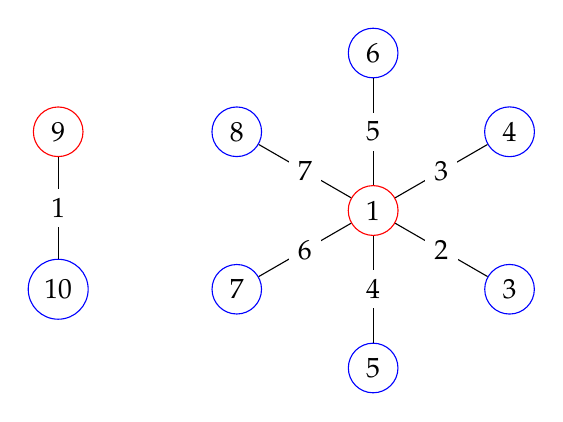
\begin{tikzpicture}[scale=2]
                % Define the vertices in a cycle
                \node (6) at (90:1) [circle, draw=blue] {6};
                \node (4) at (30:1) [circle, draw=blue] {4};
                \node (3) at (330:1) [circle, draw=blue] {3};
                \node (5) at (270:1) [circle, draw=blue] {5};
                \node (7) at (210:1) [circle, draw=blue] {7};
                \node (8) at (150:1) [circle, draw=blue] {8};
                
                % Define the center vertex
                \node (1) at (0,0) [circle, draw=red] {1};
                
                % Define the lone 2-path
                \node (9) at (-2, 0.5) [circle, draw=red] {9};
                \node (10) at (-2, -0.5) [circle, draw=blue] {10};
                
                % Draw the edges in a star
                \draw (1) -- (6) node[midway, text=black, fill=white] {5};
                \draw (1) -- (4) node[midway, text=black, fill=white] {3};
                \draw (1) -- (3) node[midway, text=black, fill=white] {2};
                \draw (1) -- (5) node[midway, text=black, fill=white] {4};
                \draw (1) -- (7) node[midway, text=black, fill=white] {6};
                \draw (1) -- (8) node[midway, text=black, fill=white] {7};
                
                % Draw the lone 2-path
                \draw (9) -- (10)node[midway, text=black, fill=white] {1};
            \end{tikzpicture}
        \end{center}
        \caption{A $\sigma^{+-}$-labeling of $S_{6}\cup P_{2}$}
    \end{figure}
    \end{frame}
    \begin{frame}{$7$ edge forest designs}
        \textbf{What about the cases where $n\equiv 7\text{ or }8\Mod{14}$?}
        \pause
        \begin{itemize}
            \item This is more complicated. $\sigma^{+-}$-labelings work because there are only lengths $\{0,\hdots,7\}$ in $K_{14}$ and so for for $K_{14t}$ we can simply increase the size of the \textcolor{blue}{B} partite set on our $\sigma^{+-}$-labeling by $7i$ for each $1\leq i\leq t$ where and then click these new labelings by $1$ to get our $G$-design of order $14t$. 
            \pause
            \item This idea also gives $G$-designs of order $14t+1$ where the new node is labeled $\infty$, and the lengths are still $\{0,\hdots,7\}$ since $\floor{\frac{15}{2}}=7$.

        \end{itemize}

    \end{frame}

    \begin{frame}{$7$ edge forest designs}
        \textbf{What about the cases where $n\equiv 7\text{ or }8\Mod{14}$?}
        \begin{itemize}
            \pause
            
            \item Lets look at the starting case we want for $K_{14t+7}$ where $t>0$ or $K_{n}$ where $n\equiv 7\Mod{14}.$ This is $K_{21}$.
            
            \item $\floor{\frac{21}{2}}=10$, so we have lengths $\{1,\hdots, 10\}$. This means we can't simply use a labeling which we click by $1$ because a $7$ edge forest can only fit $7$ distinct lengths$\hdots$
            
            \item Well, what if we can account for counting edges of some lengths $\{a,b,c\}$ from $\{1,\hdots, 10\}$? Then we can simply click some variation of our $\sigma^{+-}$-labelings accounting for lengths $\{1,\hdots,10\}\setminus \{a,b,c\}$ by $1$. 

        \end{itemize}

    \end{frame}

    \begin{frame}{Construction for $7$-edge forest designs of order $14t+7$ and $14t+8$}

        \begin{itemize} 

        \item For each forest up to isomorphism: I found three pairwise edge distinct labelings $F_{1},F_{2},F_{3}$ consisting of only lengths $\{1,2,3\}$.
        \item These labelings also had another property, which requires a new edge function: $\ell^{+}_{7}:= f(\{u,v\})= u+v \Mod{7}$. This function partitions edges by the sum of their endpoints modulo $7$. This induces a another partition on the edges: $\ell\times \ell^{+}_{7}$ where $\ell$ is the standard edge length function defined previously.
        \item Each partite set $P_{i,j}$ is the set of all edges of length $i$ with endpoint sum $j$. This gives a new way to count edges of each length, it will allow us to click by $7$ to collect all edges of any length.
        
        \end{itemize}

    \end{frame}

\begin{frame}{Construction for $7$-edge forest designs of order $14t+7$ and $14t+8$}
    \begin{itemize}
    \item Let $E_{i}$ be the set of all edges of length $i$ in $K_{21}$. Let us now take $\ell^{+}_{7}$ to be a relation between edges in the natural way. This is clearly an equivalence relation. 
    \item Then, $E_{i}\slash \ell^{+}_{7}$ the set of all equivalence classes of edges of length $i$ with respect to $\ell^{+}_{7}$; $E_{i}\slash \ell^{+}_{7}=\{[e_{0}],[e_{1}],\hdots, [e_{6}]\}$ where $\ell(e_{j})=i$ for all $0\leq j\leq 6$.
    \end{itemize}

    \textbf{An example:}

        $[\{1,2\}]_{\ell^{+}_{7}}=\{\{1,2\},\{8,9\},\{15,16\}\}$ and if we click $\{1,2\}$ by $7$ we get the whole equivalence class. The equivalence class is in fact a partite set of $\ell\times \ell^{+}_{7}$ on the edges of $K_{21}$.
\end{frame}

\begin{frame}{Construction for $7$-edge forest designs of order $14t+7$ and $14t+8$}
    \begin{itemize}
    \item So we see this equivalence relation in fact induces a group action on the edges in $E_{i}$.  We use use unions of representatives of these equivalence classes to build 'blocks' which will contain all edges of lengths $\{1,2,3\}$ of $K_{21}$ between then in order to collect all these edges and complete our design. 
    \item Recall: For each forest up to isomorphism except $S_{6}\cup P_{2}$, I found three pairwise edge distinct labelings $F_{1},F_{2},F_{3}$ consisting of only lengths $\{1,2,3\}$, with the added property that they are all pairwise $\ell\times \ell^{+}_{7}$-edge disjoint.
    \item Then, we can see that we will collect all $7$ equivalence classes for edges of lengths $1,2,3$ and clicking by $7$ all edges of lengths $1,2,3$. Then we simply adapt a $\sigma^{+-}$-labeling to contain edges of lengths $4,5,6,7,8,9,10$, and click that by $1$ to get our decompositions.
    \end{itemize}

\end{frame}

\begin{frame}{An example of such a $S_{5}\sqcup P_{3}$-design of order $21$}
    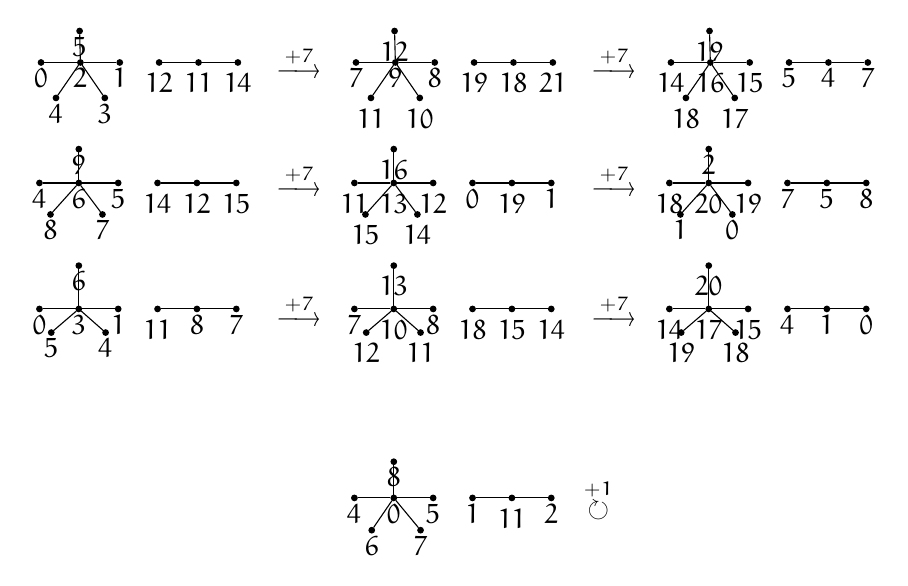
\begin{tikzpicture}[every node/.style={draw, circle, fill=black, minimum size=2pt, inner sep=0pt}]
        \node[fill=black, label=below:{\color{black}$0$}] (G1N0) at (3.72,7.33) {};
        \node[fill=black, label=below:{\color{black}$2$}] (G1N2) at (4.22,7.33) {};
        \node[fill=black, label=below:{\color{black}$1$}] (G1N1) at (4.72,7.33) {};
        \node[fill=black, label=below:{\color{black}$3$}] (G1N3) at (4.53,6.88) {};
        \node[fill=black, label=below:{\color{black}$4$}] (G1N4) at (3.91,6.88) {};
        \node[fill=black, label=below:{\color{black}$5$}] (G1N5) at (4.21,7.73) {};
        \node[fill=black, label=below:{\color{black}$12$}] (G1N12) at (5.22,7.33) {};
        \node[fill=black, label=below:{\color{black}$11$}] (G1N11) at (5.72,7.33) {};
        \node[fill=black, label=below:{\color{black}$14$}] (G1N14) at (6.22,7.33) {};
        \draw (G1N2) -- (G1N0);
        \draw (G1N2) -- (G1N1);
        \draw (G1N2) -- (G1N3);
        \draw (G1N2) -- (G1N4);
        \draw (G1N2) -- (G1N5);
        \draw (G1N12) -- (G1N11);
        \draw (G1N11) -- (G1N14);
        \node[fill=black, label=below:{\color{black}$4$}] (G2N4) at (3.70,5.80) {};
        \node[fill=black, label=below:{\color{black}$6$}] (G2N6) at (4.20,5.80) {};
        \node[fill=black, label=below:{\color{black}$5$}] (G2N5) at (4.70,5.80) {};
        \node[fill=black, label=below:{\color{black}$7$}] (G2N7) at (4.50,5.40) {};
        \node[fill=black, label=below:{\color{black}$8$}] (G2N8) at (3.84,5.40) {};
        \node[fill=black, label=below:{\color{black}$9$}] (G2N9) at (4.20,6.23) {};
        \node[fill=black, label=below:{\color{black}$14$}] (G2N14) at (5.20,5.80) {};
        \node[fill=black, label=below:{\color{black}$12$}] (G2N12) at (5.70,5.80) {};
        \node[fill=black, label=below:{\color{black}$15$}] (G2N15) at (6.20,5.80) {};
        \draw (G2N6) -- (G2N4);
        \draw (G2N6) -- (G2N5);
        \draw (G2N6) -- (G2N7);
        \draw (G2N6) -- (G2N8);
        \draw (G2N6) -- (G2N9);
        \draw (G2N14) -- (G2N12);
        \draw (G2N12) -- (G2N15);
        \node[fill=black, label=below:{\color{black}$0$}] (G3N0) at (3.70,4.20) {};
        \node[fill=black, label=below:{\color{black}$3$}] (G3N3) at (4.20,4.20) {};
        \node[fill=black, label=below:{\color{black}$1$}] (G3N1) at (4.70,4.20) {};
        \node[fill=black, label=below:{\color{black}$4$}] (G3N4) at (4.54,3.9) {};
        \node[fill=black, label=below:{\color{black}$5$}] (G3N5) at (3.85,3.9) {};
        \node[fill=black, label=below:{\color{black}$6$}] (G3N6) at (4.20,4.75) {};
        \node[fill=black, label=below:{\color{black}$11$}] (G3N11) at (5.20,4.20) {};
        \node[fill=black, label=below:{\color{black}$8$}] (G3N8) at (5.70,4.20) {};
        \node[fill=black, label=below:{\color{black}$7$}] (G3N7) at (6.20,4.20) {};
        \draw (G3N3) -- (G3N0);
        \draw (G3N3) -- (G3N1);
        \draw (G3N3) -- (G3N4);
        \draw (G3N3) -- (G3N5);
        \draw (G3N3) -- (G3N6);
        \draw (G3N11) -- (G3N8);
        \draw (G3N8) -- (G3N7);
        \begin{scope}[xshift=3cm]
            \draw[->] (3.75,7.33) -- (4.25,7.33) node[draw = none,midway, text=black, fill=white] {$\overset{+7}{\longrightarrow}$};

            \draw[->] (3.75,5.83) -- (4.25,5.83) node[draw = none,midway, text=black, fill=white] {$\overset{+7}{\longrightarrow}$};

            \draw[->] (3.75,4.18) -- (4.25,4.18) node[draw = none,midway, text=black, fill=white] {$\overset{+7}{\longrightarrow}$};
        \end{scope}

        \begin{scope}[xshift=4cm]
            
                \node[fill=black, label=below:{\color{black}$7$}] (G1N0) at (3.72,7.33) {};
                \node[fill=black, label=below:{\color{black}$9$}] (G1N2) at (4.22,7.33) {};
                \node[fill=black, label=below:{\color{black}$8$}] (G1N1) at (4.72,7.33) {};
                \node[fill=black, label=below:{\color{black}$10$}] (G1N3) at (4.53,6.88) {};
                \node[fill=black, label=below:{\color{black}$11$}] (G1N4) at (3.91,6.88) {};
                \node[fill=black, label=below:{\color{black}$12$}] (G1N5) at (4.21,7.73) {};
                \node[fill=black, label=below:{\color{black}$19$}] (G1N12) at (5.22,7.33) {};
                \node[fill=black, label=below:{\color{black}$18$}] (G1N11) at (5.72,7.33) {};
                \node[fill=black, label=below:{\color{black}$21$}] (G1N14) at (6.22,7.33) {};
                \draw (G1N2) -- (G1N0);
                \draw (G1N2) -- (G1N1);
                \draw (G1N2) -- (G1N3);
                \draw (G1N2) -- (G1N4);
                \draw (G1N2) -- (G1N5);
                \draw (G1N12) -- (G1N11);
                \draw (G1N11) -- (G1N14);
                \node[fill=black, label=below:{\color{black}$11$}] (G2N4) at (3.70,5.80) {};
                \node[fill=black, label=below:{\color{black}$13$}] (G2N6) at (4.20,5.80) {};
                \node[fill=black, label=below:{\color{black}$12$}] (G2N5) at (4.70,5.80) {};
                \node[fill=black, label=below:{\color{black}$14$}] (G2N7) at (4.50,5.40) {};
                \node[fill=black, label=below:{\color{black}$15$}] (G2N8) at (3.84,5.40) {};
                \node[fill=black, label=below:{\color{black}$16$}] (G2N9) at (4.20,6.23) {};
                \node[fill=black, label=below:{\color{black}$0$}] (G2N14) at (5.20,5.80) {};
                \node[fill=black, label=below:{\color{black}$19$}] (G2N12) at (5.70,5.80) {};
                \node[fill=black, label=below:{\color{black}$1$}] (G2N15) at (6.20,5.80) {};
                \draw (G2N6) -- (G2N4);
                \draw (G2N6) -- (G2N5);
                \draw (G2N6) -- (G2N7);
                \draw (G2N6) -- (G2N8);
                \draw (G2N6) -- (G2N9);
                \draw (G2N14) -- (G2N12);
                \draw (G2N12) -- (G2N15);
                \node[fill=black, label=below:{\color{black}$7$}] (G3N0) at (3.70,4.20) {};
                \node[fill=black, label=below:{\color{black}$10$}] (G3N3) at (4.20,4.20) {};
                \node[fill=black, label=below:{\color{black}$8$}] (G3N1) at (4.70,4.20) {};
                \node[fill=black, label=below:{\color{black}$11$}] (G3N4) at (4.54,3.9) {};
                \node[fill=black, label=below:{\color{black}$12$}] (G3N5) at (3.85,3.9) {};
                \node[fill=black, label=below:{\color{black}$13$}] (G3N6) at (4.20,4.75) {};
                \node[fill=black, label=below:{\color{black}$18$}] (G3N11) at (5.20,4.20) {};
                \node[fill=black, label=below:{\color{black}$15$}] (G3N8) at (5.70,4.20) {};
                \node[fill=black, label=below:{\color{black}$14$}] (G3N7) at (6.20,4.20) {};
                \draw (G3N3) -- (G3N0);
                \draw (G3N3) -- (G3N1);
                \draw (G3N3) -- (G3N4);
                \draw (G3N3) -- (G3N5);
                \draw (G3N3) -- (G3N6);
                \draw (G3N11) -- (G3N8);
                \draw (G3N8) -- (G3N7);
                \node[fill=black, label=below:{\color{black}$4$}] (G4N4) at (3.70,1.80) {};
        \node[fill=black, label=below:{\color{black}$0$}] (G4N0) at (4.20,1.80) {};
        \node[fill=black, label=below:{\color{black}$5$}] (G4N5) at (4.70,1.80) {};
        \node[fill=black, label=below:{\color{black}$6$}] (G4N6) at (3.92,1.39) {};
        \node[fill=black, label=below:{\color{black}$7$}] (G4N7) at (4.54,1.39) {};
        \node[fill=black, label=below:{\color{black}$8$}] (G4N8) at (4.20,2.26) {};
        \node[fill=black, label=below:{\color{black}$1$}] (G4N1) at (5.20,1.80) {};
        \node[fill=black, label=below:{\color{black}$11$}] (G4N11) at (5.70,1.80) {};
        \node[fill=black, label=below:{\color{black}$2$}] (G4N2) at (6.20,1.80) {};
        \draw (G4N0) -- (G4N4);
        \draw (G4N0) -- (G4N5);
        \draw (G4N0) -- (G4N6);
        \draw (G4N0) -- (G4N7);
        \draw (G4N0) -- (G4N8);
        \draw (G4N1) -- (G4N11);
        \draw (G4N11) -- (G4N2);
        
            \draw[->] (6.8,1.78) -- (6.8,1.78) node[draw = none,midway, text=black, fill=white] {$\overset{+1}{\circlearrowright}$};

        \end{scope}
        \begin{scope}[xshift=7cm]
            \draw[->] (3.75,7.33) -- (4.25,7.33) node[draw = none,midway, text=black, fill=white] {$\overset{+7}{\longrightarrow}$};

            \draw[->] (3.75,5.83) -- (4.25,5.83) node[draw = none,midway, text=black, fill=white] {$\overset{+7}{\longrightarrow}$};

            \draw[->] (3.75,4.18) -- (4.25,4.18) node[draw = none,midway, text=black, fill=white] {$\overset{+7}{\longrightarrow}$};
        \end{scope}
        \begin{scope}[xshift = 8cm]

                \node[fill=black, label=below:{\color{black}$14$}] (G1N0) at (3.72,7.33) {};
                \node[fill=black, label=below:{\color{black}$16$}] (G1N2) at (4.22,7.33) {};
                \node[fill=black, label=below:{\color{black}$15$}] (G1N1) at (4.72,7.33) {};
                \node[fill=black, label=below:{\color{black}$17$}] (G1N3) at (4.53,6.88) {};
                \node[fill=black, label=below:{\color{black}$18$}] (G1N4) at (3.91,6.88) {};
                \node[fill=black, label=below:{\color{black}$19$}] (G1N5) at (4.21,7.73) {};
                \node[fill=black, label=below:{\color{black}$5$}] (G1N12) at (5.22,7.33) {};
                \node[fill=black, label=below:{\color{black}$4$}] (G1N11) at (5.72,7.33) {};
                \node[fill=black, label=below:{\color{black}$7$}] (G1N14) at (6.22,7.33) {};
                \draw (G1N2) -- (G1N0);
                \draw (G1N2) -- (G1N1);
                \draw (G1N2) -- (G1N3);
                \draw (G1N2) -- (G1N4);
                \draw (G1N2) -- (G1N5);
                \draw (G1N12) -- (G1N11);
                \draw (G1N11) -- (G1N14);
                \node[fill=black, label=below:{\color{black}$18$}] (G2N4) at (3.70,5.80) {};
                \node[fill=black, label=below:{\color{black}$20$}] (G2N6) at (4.20,5.80) {};
                \node[fill=black, label=below:{\color{black}$19$}] (G2N5) at (4.70,5.80) {};
                \node[fill=black, label=below:{\color{black}$0$}] (G2N7) at (4.50,5.40) {};
                \node[fill=black, label=below:{\color{black}$1$}] (G2N8) at (3.84,5.40) {};
                \node[fill=black, label=below:{\color{black}$2$}] (G2N9) at (4.20,6.23) {};
                \node[fill=black, label=below:{\color{black}$7$}] (G2N14) at (5.20,5.80) {};
                \node[fill=black, label=below:{\color{black}$5$}] (G2N12) at (5.70,5.80) {};
                \node[fill=black, label=below:{\color{black}$8$}] (G2N15) at (6.20,5.80) {};
                \draw (G2N6) -- (G2N4);
                \draw (G2N6) -- (G2N5);
                \draw (G2N6) -- (G2N7);
                \draw (G2N6) -- (G2N8);
                \draw (G2N6) -- (G2N9);
                \draw (G2N14) -- (G2N12);
                \draw (G2N12) -- (G2N15);
                \node[fill=black, label=below:{\color{black}$14$}] (G3N0) at (3.70,4.20) {};
                \node[fill=black, label=below:{\color{black}$17$}] (G3N3) at (4.20,4.20) {};
                \node[fill=black, label=below:{\color{black}$15$}] (G3N1) at (4.70,4.20) {};
                \node[fill=black, label=below:{\color{black}$18$}] (G3N4) at (4.54,3.9) {};
                \node[fill=black, label=below:{\color{black}$19$}] (G3N5) at (3.85,3.9) {};
                \node[fill=black, label=below:{\color{black}$20$}] (G3N6) at (4.20,4.75) {};
                \node[fill=black, label=below:{\color{black}$4$}] (G3N11) at (5.20,4.20) {};
                \node[fill=black, label=below:{\color{black}$1$}] (G3N8) at (5.70,4.20) {};
                \node[fill=black, label=below:{\color{black}$0$}] (G3N7) at (6.20,4.20) {};
                \draw (G3N3) -- (G3N0);
                \draw (G3N3) -- (G3N1);
                \draw (G3N3) -- (G3N4);
                \draw (G3N3) -- (G3N5);
                \draw (G3N3) -- (G3N6);
                \draw (G3N11) -- (G3N8);
                \draw (G3N8) -- (G3N7);
                
        
        \end{scope}
        \end{tikzpicture}
\end{frame}

\begin{frame}{Summary}
\begin{itemize}
\item Notice that that there are no wrap-around edges in this decomposition. This means we can click the graphs in the first column of the previous figure by $7$ a total of $|7|$ in $\ZZ_{14t+7}$ for any $t>0$ to get all length $1,2,3$ edges in $K_{14t+7}$
\item Then we do the same thing we did for $\sigma^{+-}$-labelings with the graph in the fourth row, just make copies of it for the next new edge lengths for each $t$ and click all those by $1$
\item We simply add one more labeling for $K_{14t+8}$ and a new edge length $\infty$ that goes with the new $\infty$ node.
\item We had to take a different combinatorial approach for $S_{6}\sqcup P_{2}$ where we broke off edges from $7$-star decompositions of $K_{21}$ proven to exist by P. Cain in 1974.
\end{itemize}
\end{frame}

\begin{frame}{Thank you!}
    \textbf{What's left?}
    \begin{itemize}
    \item I still have to finish the labelings for $K_{22}$ which give the decomposition for $K_{14t+8}$ where $t>0$. Going smoothly.
    \item We have to prove we can break off edges for all graphs in the design constructions by P. Cain to get our $S_{6}\sqcup P_{2}$-designs.
    \item Once done with the above we can probably extend this strategy to other 7 edge graphs to complete all 7-edge designs of order $n$. There are similar labelings to $\sigma^{+-}$ and our approach to the other idempotent $n$'s are not family specific. 
    \end{itemize}
\begin{center}
    \textbf{Thank you all for coming!}
\end{center}

    \end{frame}

\end{document}
